\section{Implementación}
\label{sec:implementacion}

Una vez establecidos los requisitos cubiertos en el Trabajo Fin de Grado (\referenciaSeccion{sec:requisitos}) y estipulados los cambios y la definición de la arquitectura de la aplicación en general y de cada componente en particular (\referenciaSeccion{sec:diseñoArquitectura}), la presente sección pretende describir el proceso de implementación de algunos requisitos, desarrollando cómo se ha procedido a la creación y modificación de código para su consecución.

Las siguientes páginas introducen una descripción pormenorizada de los requerimientos implementados más destacados, organizándolos en subsecciones según las categorías de requisitos establecidas en la enumeración anteriormente referenciada.

\subsection{Requisitos funcionales}
\label{subsec:reqsFuncionales}
\subsubsection{\texttt{RF-1}: registro de profesores por invitación}
\label{subsec:rf1}

En la versión de \textit{VSCode4Teaching} tomada como punto de partida, mientras que los estudiantes gozaban de libertad total para poder crear una cuenta en la aplicación a través de la extensión, los profesores debían ser registrados manualmente por otros profesores, evitando así que estudiantes o personal no acreditado pudiese tener cuenta con privilegios de docente. Esto conllevaba que los profesores con cuenta preexistente tuviesen que introducir manualmente el nombre, apellidos, correo electrónico, nombre de usuario y contraseña de los nuevos docentes, generando un riesgo de seguridad ---ya que no es posible modificar la contraseña una vez establecida---.

Como consecuencia, se ha modificado este proceso para ``invertir'' su funcionamiento, de modo que los profesores pueden generar invitaciones para otros docentes introduciendo su nombre, apellidos, correo electrónico y nombre de usuario. Una vez generada la invitación, que tiene forma de enlace a una página web ---con el aspecto visual reflejado en la \referenciaFigura{fig:reqf1-1}---, puede remitírsela al docente invitado, quien puede acceder al enlace en un navegador web para, introduciendo su nombre de usuario como método de verificación, escoger la contraseña de su elección sin necesidad de comunicársela a ninguna otra persona.

Esta es una de las funcionalidades que aprovecha la introducción de la nueva aplicación web SPA introducida como cliente adicional del servidor ---tal como figura en la \referenciaSeccion{sec:diseñoArquitectura}---, ya que el docente invitado accede mediante el enlace suministrado a un asistente implementado dentro de esta aplicación web ---y no en la extensión---.

\begin{figure}[ht]
    \centering
    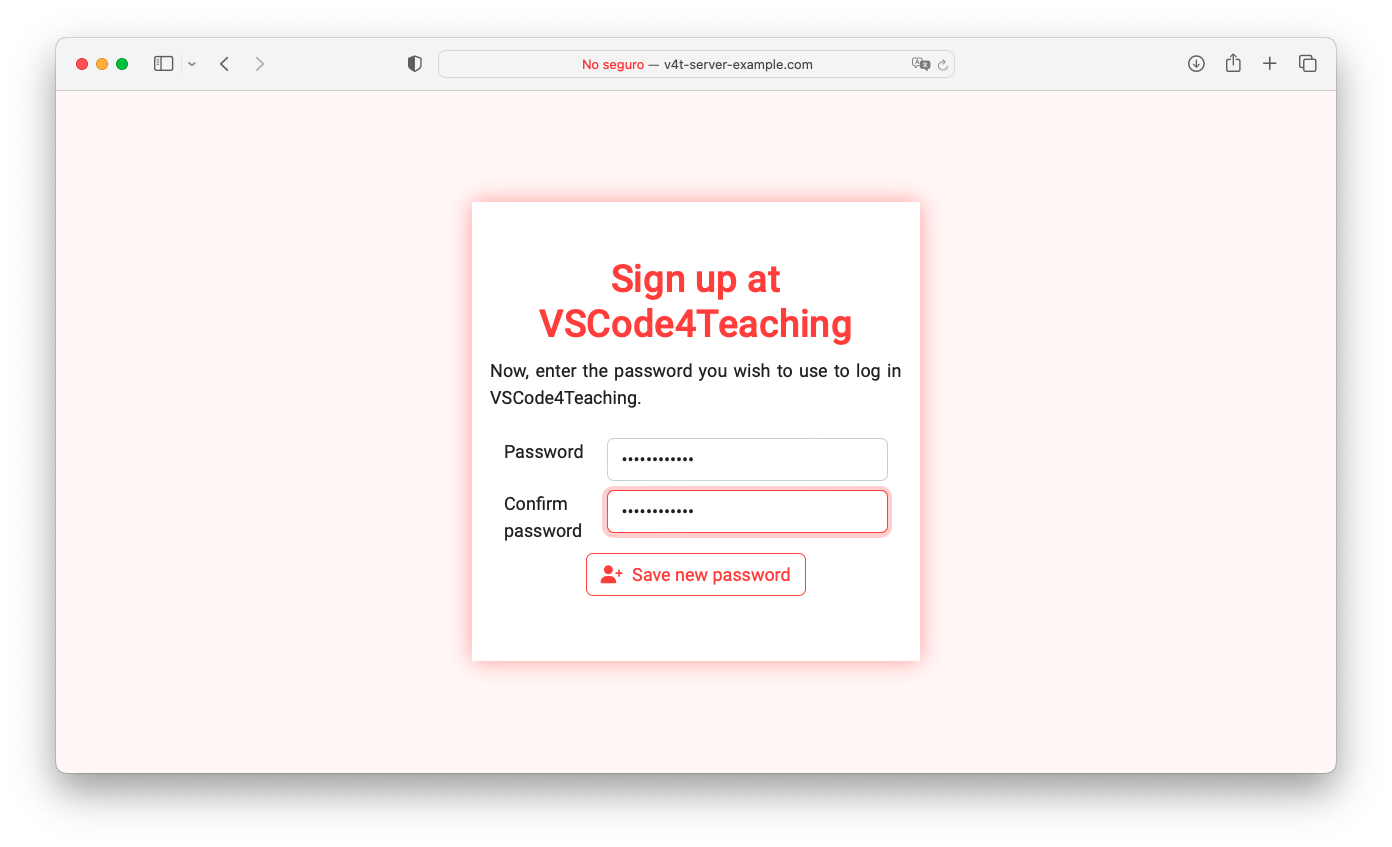
\includegraphics[width=\textwidth]{imagenes/utilizadas/4-3-implementacion/rf1-1.png}
    \caption{Captura del navegador web durante el proceso de configuración de contraseña de un nuevo profesor.}
    \label{fig:reqf1-1}
\end{figure}

\subsubsection{\texttt{RF-2}: alta simultánea de ejercicios}
\label{subsec:rf2}

Uno de los procesos más habitualmente repetidos en \textit{VSCode4Teaching} es, desde su primera versión, la subida o adición de nuevos ejercicios dentro de los cursos por parte de los profesores. Este proceso requería necesariamente rellenar un campo de texto con el nombre del ejercicio y seleccionar el fichero, directorio o conjunto de ambos que conformaba la plantilla, subiéndola al servidor y proporcionándosela al alumnado cuando descargasen el ejercicio por primera vez para tomarla como base de su propia propuesta de resolución.

La implementación de este requisito busca crear una nueva forma de subir los ejercicios que simplifique el proceso anteriormente descrito y permita, además, añadir varios ejercicios de una sola vez. En la \referenciaFigura{fig:reqf2-1} se muestra una captura de la extensión en la que se señala el botón para añadir un solo ejercicio (en verde) y el nuevo botón que da acceso a la funcionalidad para subir varios ejercicios en una sola acción (en naranja).

Gracias a la incorporación de esta nueva funcionalidad, los profesores pueden subir varios ejercicios de forma simultánea seleccionando un directorio que tenga en su interior una carpeta para cada ejercicio que se desea crear, de forma que se toma el nombre de cada directorio como el del nuevo ejercicio ---siendo modificable posteriormente---; y sus contenidos, como la plantilla del ejercicio (y la solución, en caso de incluirla, tal como se refleja en la \referenciaSeccion{subsec:rf5}).

\begin{figure}[ht]
    \centering
    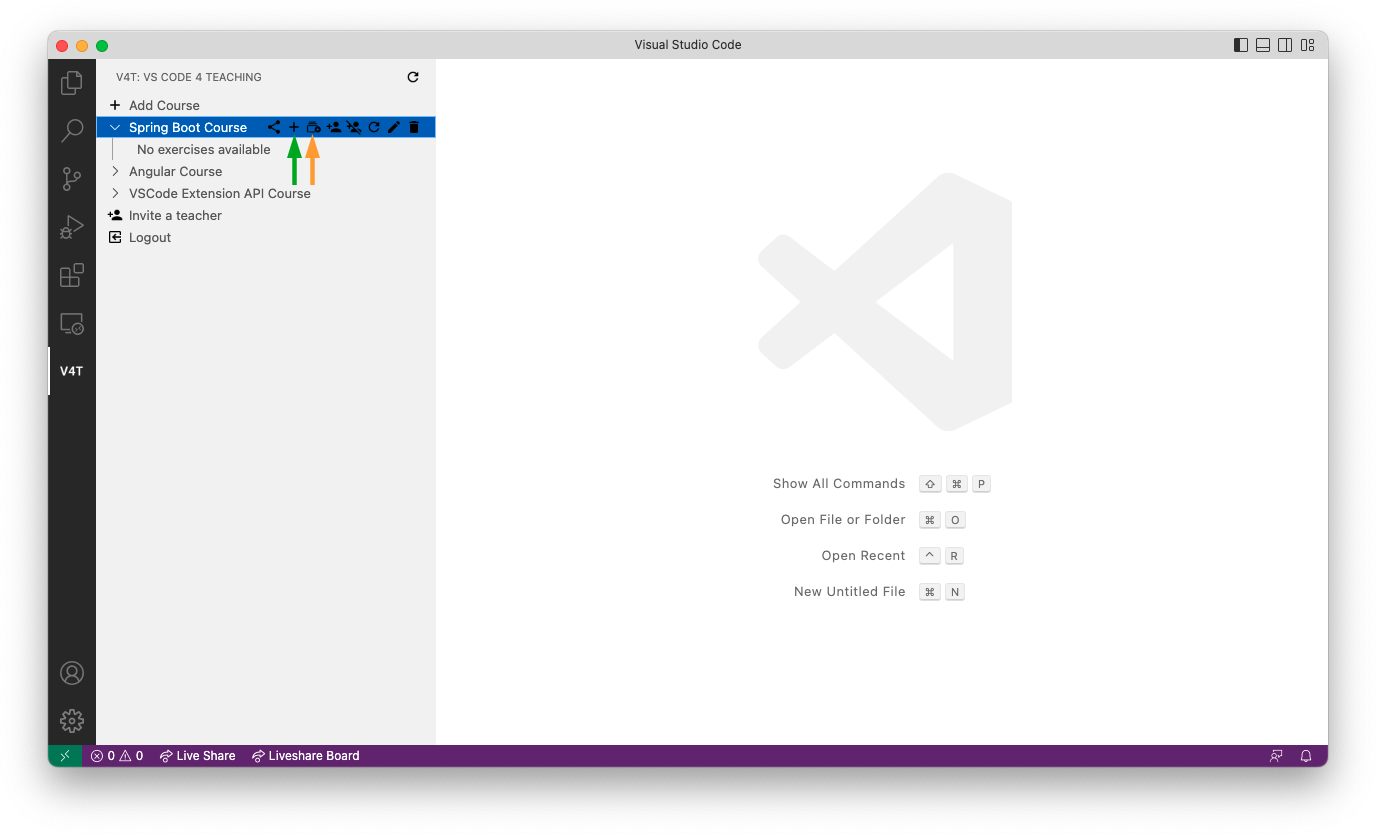
\includegraphics[width=0.975\textwidth]{imagenes/utilizadas/4-3-implementacion/rf2-1.png}
    \caption{Captura de la extensión en la que se destacan los botones empleados para añadir ejercicios.}
    \label{fig:reqf2-1}
\end{figure}

\subsubsection{\texttt{RF-3}: anonimato de propuestas de estudiantes}
\label{subsec:rf3}

Cuando un profesor descargaba un ejercicio en las primeras versiones de \textit{VSCode4Teaching}, la estructura de ficheros que se habilitaba en su entorno de desarrollo incluía un directorio ``template'' con la plantilla original del ejercicio y tantos directorios como propuestas de alumnos terminadas o parcialmente guardadas hubiese, identificando cada una de ellas con el nombre de usuario del alumno. Además, el \textit{dashboard} ---creado para que los profesores pudieran obtener información del progreso de sus estudiantes en la realización de los ejercicios--- incluía como elemento principal una tabla que reflejaba nombre, apellidos, nombre de usuario y fecha de última modificación para cada uno de los estudiantes del curso.

En cumplimiento del primer objetivo de los recogidos en el \referenciaCapitulo{cap:objetivos}, la presente tarea conduce a la modificación de los mecanismos de identificación de las propuestas de resolución de los ejercicios remitidas por los estudiantes con el fin de poder garantizar su anonimato. Para ello, se introducen dos requisitos derivados:

\begin{itemize}
    \item El requisito \texttt{RF-3.1} establece la necesidad de alterar el sistema de nomenclatura que se emplea para almacenar las propuestas enviadas por los estudiantes. Como consecuencia, se introduce una modificación por la que el servidor asigna como nombre del directorio de cada una de ellas un texto del formato ``student\_\texttt X'', siendo \texttt X el número identificador de la propuesta almacenado en base de datos. Este formato permite cotejar el número empleado para formar el nombre del directorio (\texttt X) con los datos persistidos, pudiendo así relacionar la propuesta de cada estudiante con su propia información de forma rápida. La \referenciaFigura{fig:reqf3-1} recoge una comparativa entre los formatos anterior y actual.
    \item El requisito \texttt{RF-3.2} estipula las dos actuaciones que se ejecutan sobre el \textit{dashboard}: la modificación de la columna que recoge el nombre de usuario de los estudiantes, introduciendo en ella el nombre del directorio que recoge su propuesta de solución; y la introducción de un elemento de control interactivo que permita a los docentes ocultar o mostrar la columna de nombres y apellidos a elección. En la \referenciaFigura{fig:reqf3-2} se destaca este elemento de control y se puede visualizar la tabla sin y con la mencionada columna cuando este está activado y desactivado, respectivamente.
\end{itemize}

De este modo, la ejecución de ambos requisitos permite lograr una situación de total anonimato de los estudiantes si así lo desea el docente, pudiendo relacionar cada nombre de directorio con el nombre propio y los apellidos de cada estudiante en el \textit{dashboard} cuando lo desee.

\begin{figure}[ht]
    \centering
    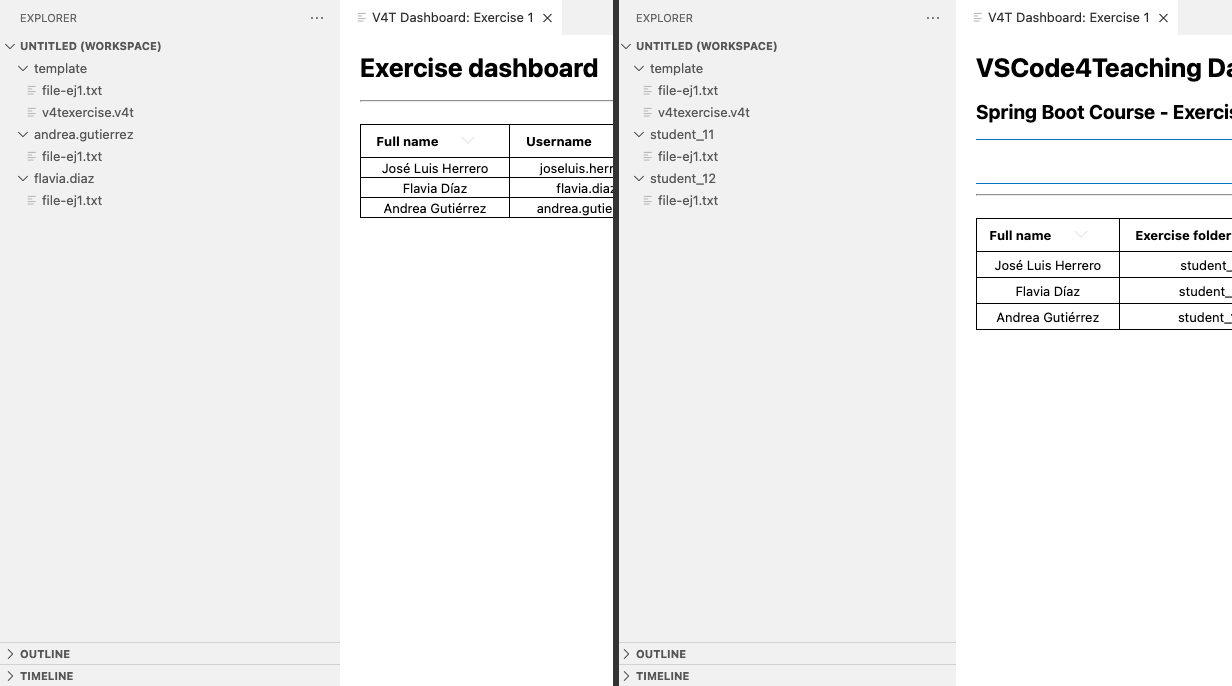
\includegraphics[width=\textwidth]{imagenes/utilizadas/4-3-implementacion/rf3-1.png}
    \caption{Comparativa entre los formatos anterior (izquierda) y actual (derecha) de almacenamiento de propuestas de estudiantes.}
    \label{fig:reqf3-1}
\end{figure}

\begin{figure}[ht]
    \centering
    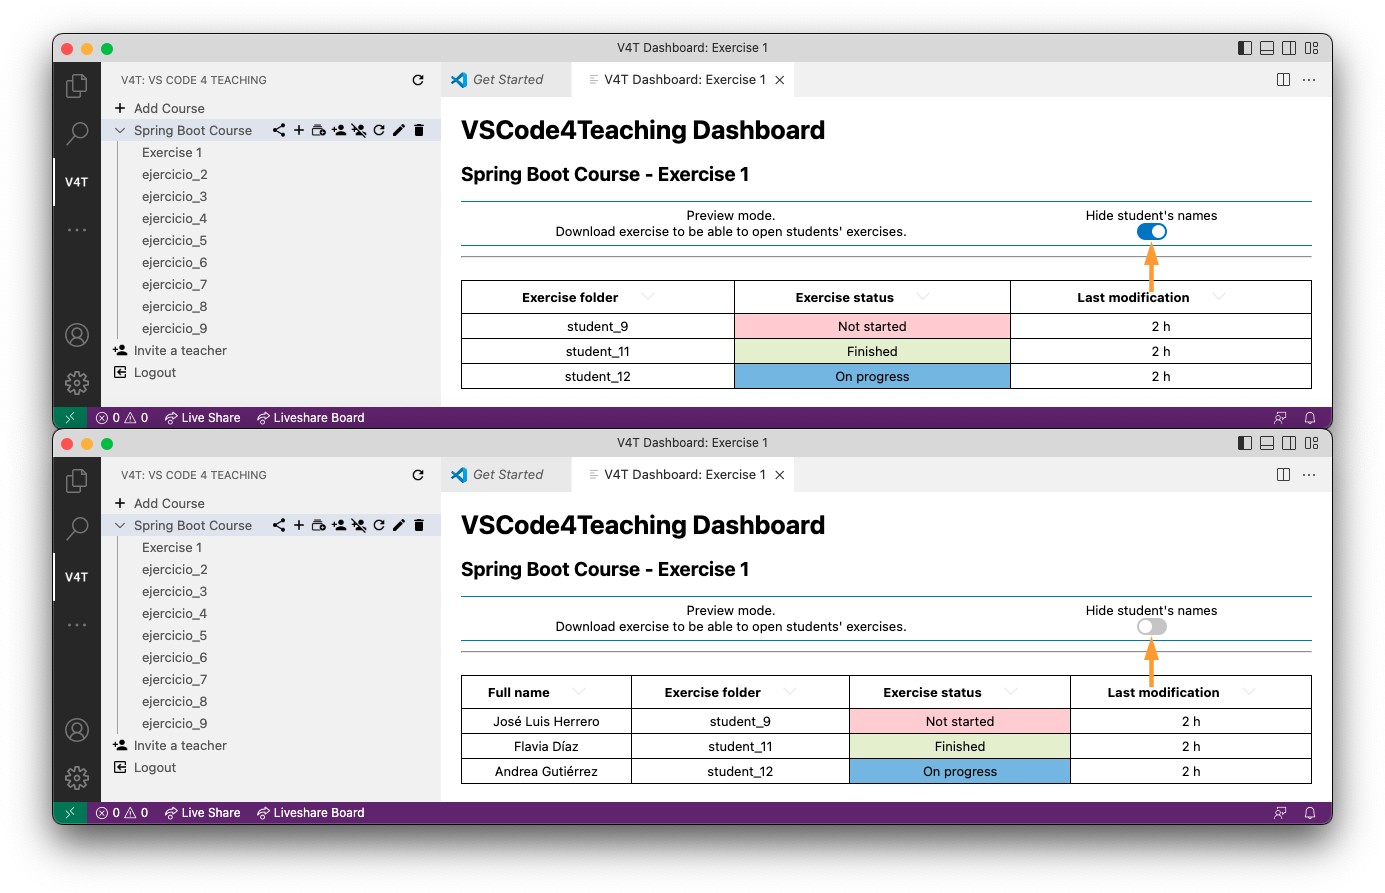
\includegraphics[width=0.975\textwidth]{imagenes/utilizadas/4-3-implementacion/rf3-2.png}
    \caption{Captura de la extensión en la que se destaca el nuevo elemento para ocultar y mostrar la identidad de los estudiantes.}
    \label{fig:reqf3-2}
\end{figure}

\subsubsection{\texttt{RF-4}: previsualización del \textit{dashboard}}
\label{subsec:rf4}

La versión de \textit{VSCode4Teaching} tomada como punto de partida para el inicio del presente TFG incluía ya un \textit{dashboard} completamente funcional que requería que el profesor tuviese descargado el ejercicio completo en su propio espacio de trabajo en Visual Studio Code para poder ejecutar las funcionalidades de apertura de ficheros y visualización de diferencias con la plantilla, que se ejecutan mediante botones situados en cada fila de la tabla mostrada en esta visualización.

El presente requisito busca eliminar la necesidad de descargar todos los ficheros de los ejercicios y permitir a los profesores visualizar el \textit{dashboard} ---sin acceso a las funcionalidades anteriormente nombradas--- para el ejercicio que deseen con independencia del que tengan activo en su espacio de trabajo. Este formato de ``previsualización'' conlleva modificaciones del \textit{dashboard}, que únicamente deberá mostrar la columna con las acciones anteriormente citadas si se abre en ``modo completo'' ---es decir, tal como se venía haciendo en versiones anteriores---. Los profesores pueden acceder a la previsualización del \textit{dashboard} de cada ejercicio haciendo uso de un nuevo botón colocado en la barra lateral junto a cada ejercicio, tal como se puede evidenciar en la \referenciaFigura{fig:reqf4-1}. Esta previsualización introduce, además, un elemento gráfico explicativo que aclara al profesor que, en caso de querer ejecutar las acciones de apertura y visualización de diferencias entre archivos, deberá descargar el ejercicio y hacer uso del \textit{dashboard} completo.

\begin{figure}[ht]
    \centering
    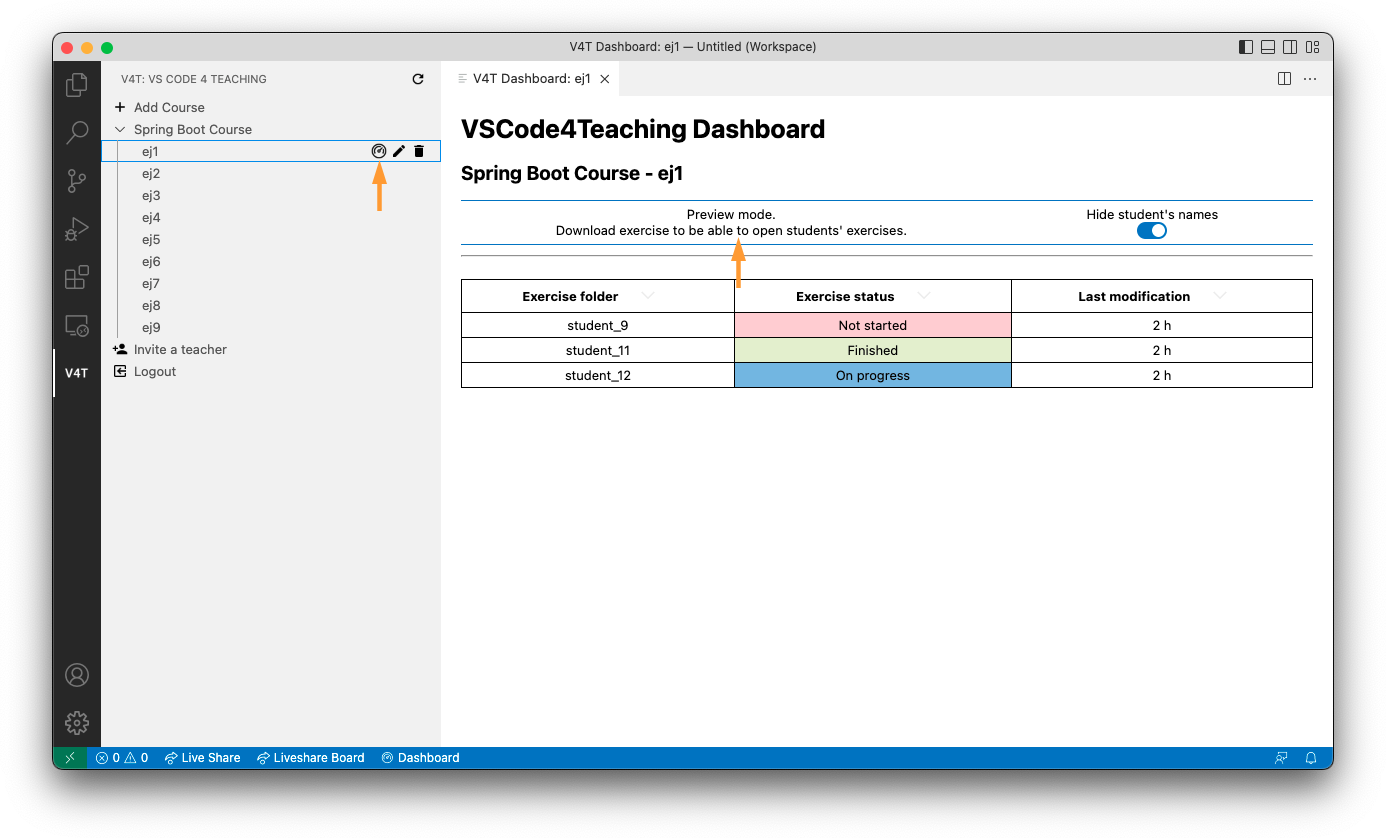
\includegraphics[width=\textwidth]{imagenes/utilizadas/4-3-implementacion/rf4-1.png}
    \caption{Captura de la extensión en la que se muestran los elementos de la GUI que permiten distinguir el modo de previsualización del \textit{dashboard}.}
    \label{fig:reqf4-1}
\end{figure}

\subsubsection{\texttt{RF-5}: guardado de soluciones de ejercicios}
\label{subsec:rf5}

Uno de los objetivos principales fijados para la evolución del proyecto \textit{VSCode4Teaching} es, tal como queda reflejado en el tercer punto del \referenciaCapitulo{cap:objetivos}, permitir al profesorado adjuntar a los ejercicios su propia propuesta de resolución, que sería accesible a los estudiantes una vez fuese publicada. Este requisito, junto con los requerimientos \texttt{RF-6}, \texttt{RF-7} y \texttt{RF-8} ---desarrollados en sendos apartados posteriores---, da cumplimiento al citado objetivo.

Con anterioridad a la implementación de este requisito, la aplicación permitía a los docentes añadir nuevos ejercicios ---tanto de uno en uno como de forma múltiple---, adjuntando a cada uno su correspondiente plantilla. Una vez implementado, se requiere a los usuarios que proporcionen un directorio por cada ejercicio y, si desean introducir solución asociada, que este contenga únicamente dos carpetas en su interior: ``template'', que recoja todos los contenidos relativos a la plantilla del ejercicio; y ``solution'', que albergue la totalidad de la propuesta de solución que se ha de adjuntar al nuevo ejercicio. Todas las estructuras distintas a la anteriormente descrita se interpretarán como plantillas incluidas para ejercicios sin solución adjunta.

La implementación de la posibilidad de incluir una solución ha tomado como base la capacidad anteriormente existente para albergar plantillas, conllevando las siguientes alteraciones:
\begin{itemize}
    \item Se ha modificado el modelo de dominio asociado a los ejercicios en el servidor para introducir la persistencia en base de datos de la información relativa a la solución siguiendo el modelo empleado para las plantillas. Asimismo, se han modificado los modelos de dominio asociados a los ejercicios en el servidor y en el cliente para introducir un valor \textit{booleano}\footnote{Booleano. También conocido como binario, es un tipo de dato que permite albergar únicamente dos posibles valores: verdadero o falso.} que almacena si un ejercicio tiene o no solución (independientemente de su disponibilidad).
    \item Se ha aprovechado el código existente para la subida de plantillas y de propuestas de estudiantes al servidor para, unificando procedimientos y eliminando bloques de código repetidos, añadir un nuevo \textit{endpoint} a la API REST para la subida de las soluciones.
    \item Se ha implementado un algoritmo en la extensión que, dado un directorio, se basa en la exploración de los contenidos de la ruta local proporcionada para determinar si la estructura de ficheros que contiene es la requerida para incluir solución o no en el momento de subir el ejercicio.
\end{itemize}

\subsubsection{\texttt{RF-6}: configuración de soluciones para profesores}
\label{subsec:rf6}

Uno de los objetivos principales fijados para la evolución del proyecto es permitir al profesorado adjuntar a los ejercicios su propia propuesta de resolución, que será accesible a los estudiantes una vez sea publicada. Este requisito es uno de los que busca dar cumplimiento al objetivo tercero del \referenciaCapitulo{cap:objetivos}.

El presente requerimiento tiene como fin la incorporación de controles que permitan a los profesores determinar cuándo es pública una solución y si los estudiantes pueden (o no) hacer modificaciones a sus propuestas propias de resolución de los ejercicios una vez hayan accedido a la solución propuesta por el docente.

De este modo, las soluciones permanecen ocultas por defecto a los estudiantes hasta que el profesor decida publicarlas, siendo este cambio irreversible; esto es, una vez publicada no puede ser despublicada. Por otro lado, el comportamiento por defecto de la aplicación es el de bloquear la edición de los ejercicios una vez el estudiante descargue la propuesta de solución del docente, pasándolo a estado ``finalizado'' automáticamente cuando el estudiante inicie la descarga de la solución, previa solicitud de confirmación. Si el docente lo desea, puede modificar este comportamiento, de modo que el estado permanecerá con el valor ``en progreso'' a pesar de haber descargado la solución, considerando que este ajuste debe estar adecuadamente configurado antes de la publicación de la solución, ya que este parámetro también permanecerá inmutable tras publicarla. Ambas modificaciones de configuración se pueden realizar a través del \textit{dashboard} de los ejercicios que tienen solución, tal como se puede apreciar en la \referenciaFigura{fig:reqf6-1}.

Para efectuar esta implementación, se han realizado los siguientes cambios:
\begin{itemize}
    \item Se han alterado los modelos de dominio de la entidad relativa a los ejercicios tanto en el servidor como en el cliente para introducir dos valores \textit{booleanos} para controlar la disponibilidad de la solución y la capacidad de edición tras su descarga.
    \item Se han introducido dos elementos de interacción de usuario en forma de casillas de verificación para dotar al profesorado de la capacidad para modificar los atributos de configuración descritos con anterioridad. Estos elementos quedan señalados en la figura anteriormente referenciada.
\end{itemize}

\begin{figure}[ht]
    \centering
    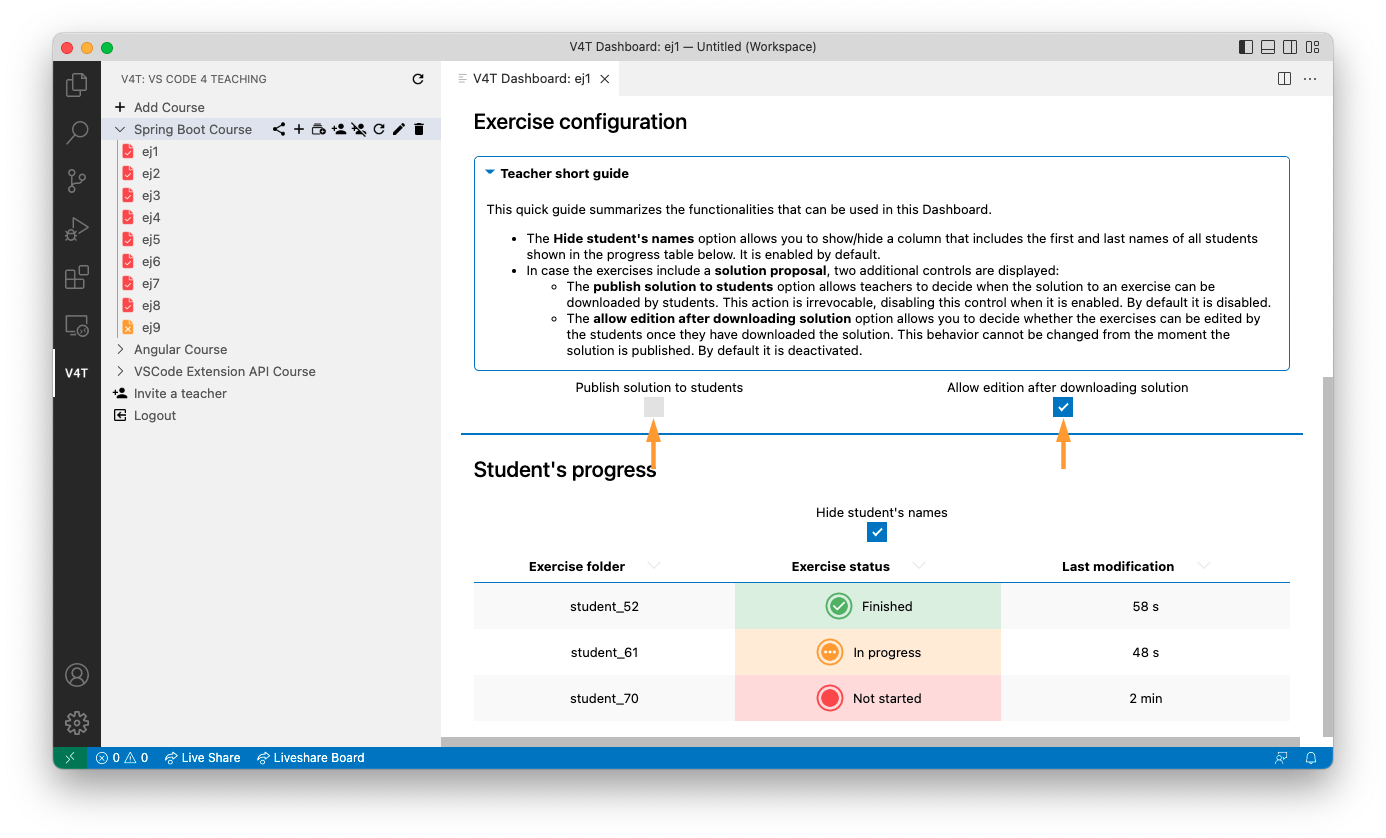
\includegraphics[width=\textwidth]{imagenes/utilizadas/4-3-implementacion/rf6-1.png}
    \caption{Captura de la extensión en la que se destacan los elementos gráficos para la modificación de la configuración de la solución de un ejercicio.}
    \label{fig:reqf6-1}
\end{figure}

\subsubsection{\texttt{RF-7}: descarga de soluciones}
\label{subsec:rf7}

Tal como se introduce en los dos epígrafes anteriores, uno de los objetivos principales fijados para la evolución del proyecto es permitir a los estudiantes descargar las propuestas de solución adjuntadas por el profesorado a los ejercicios realizados siempre y cuando hayan sido publicadas por ellos.

Este requerimiento afecta a profesores y a estudiantes de forma diferente, por lo que da lugar a en dos requisitos según el rol:
\begin{itemize}
    \item El requisito \texttt{RF-7.1} establece que los estudiantes deben poder tener acceso a la descarga de la solución de un ejercicio siempre que exista solución y que haya sido publicada por los profesores.
    
    Para incorporar este punto, se ha aprovechado la implementación del requisito \texttt{RF-7.2}, introduciendo un control específico para usuarios con rol de estudiantes sobre la disponibilidad de la solución. En caso de que se den las condiciones adecuadas, se habilita un nuevo botón para la descarga de la solución y se lanza un aviso en la parte inferior del entorno de desarrollo, tal como ilustra la \referenciaFigura{fig:reqf7-1}.

    Al presionar el botón, aparece un cuadro de diálogo modal que informa al estudiante acerca de si tendrá la capacidad de editar posteriormente su ejercicio o si se marcará automáticamente como ``finalizado'' tras descargar la solución. Una vez el estudiante confirme que desee continuar, la solución se descargará y situará en un nuevo directorio llamado ``solution'' ubicado en el nivel inmediatamente inferior al del directorio padre del ejercicio activo.

    Adicionalmente, se han ampliado las capacidades del botón de refresco de la extensión y, en caso de que haya un ejercicio activo, la acción desencadenada por su utilización también verificará si la solución ha sido publicada desde la última vez que se descargó el ejercicio, favoreciendo la usabilidad de esta funcionalidad de modo que los estudiantes no tengan que desactivar y volver a acceder un ejercicio para comprobar si la solución ya es pública.
    \item El requisito \texttt{RF-7.2} determina que los profesores deben tener acceso a la solución que han adjuntado a sus propios ejercicios ---en caso de haberla---, descargándose junto con la plantilla y las propuestas de resolución parciales o finales de los estudiantes al activar un ejercicio desde la extensión.
    
    Para ejecutar la implementación de este requisito, se han tomado como ejemplo los métodos y procedimientos dispuestos tanto en servidor como en cliente para la descarga de la plantilla, reutilizando el código ---y previniendo la aparición de duplicidades--- para la implementación de esta capacidad. Como consecuencia, la solución se descarga en paralelo a la plantilla para los profesores independientemente de su estado de publicación.
\end{itemize}

\begin{figure}[ht]
    \centering
    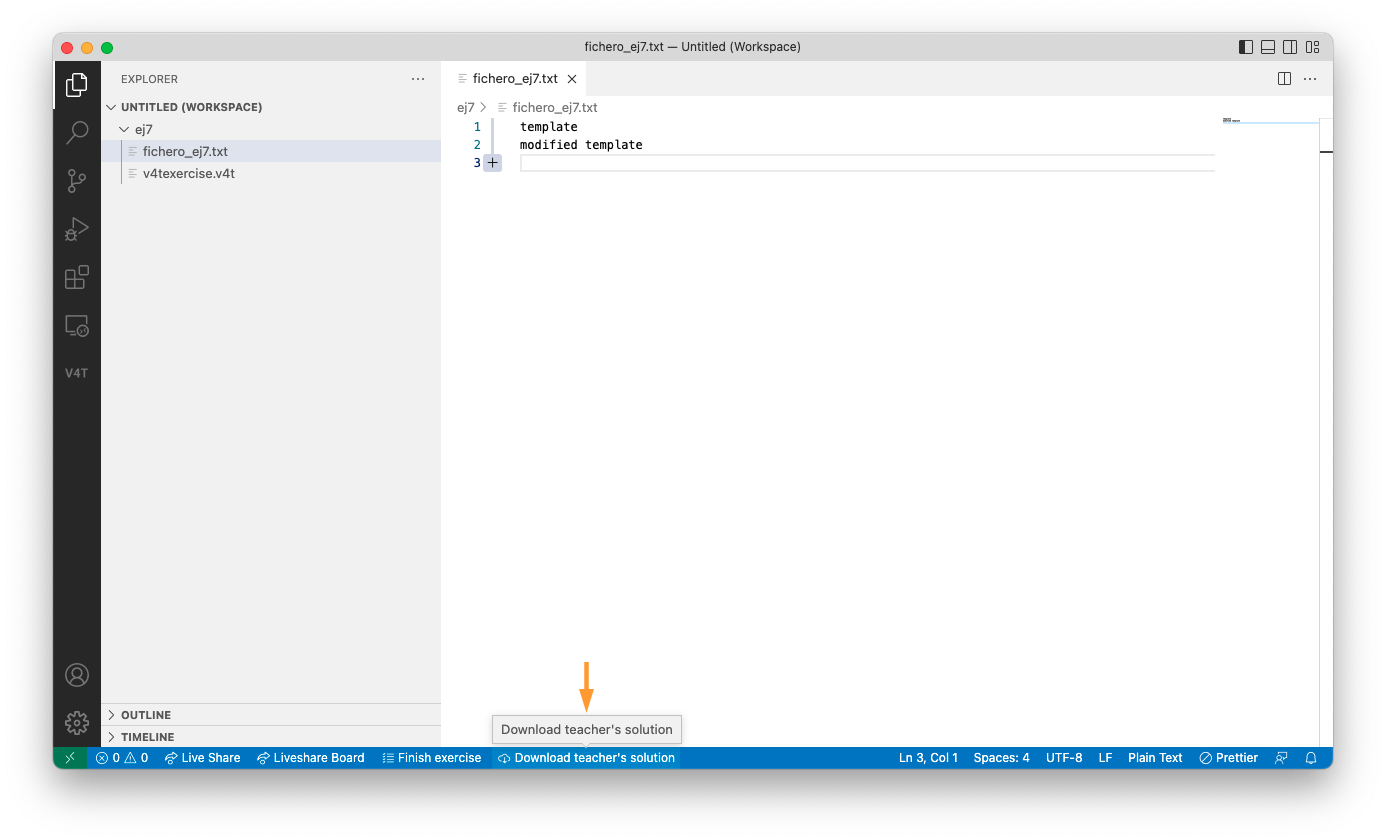
\includegraphics[width=\textwidth]{imagenes/utilizadas/4-3-implementacion/rf7-1.png}
    \caption{Captura de la extensión en la que se destaca el botón habilitado para la descarga de soluciones a ejercicios.}
    \label{fig:reqf7-1}
\end{figure}

\subsubsection{\texttt{RF-8}: visualización de diferencias con solución}
\label{subsec:rf8}

Este requisito busca completar el objetivo del \texttt{RF-7.1} ---\referenciaSeccion{subsec:rf7}---, por el que se permite a los estudiantes descargar las soluciones de los ejercicios que dispongan de ella a partir de su publicación por parte del profesor.

El presente requerimiento aborda la creación de una característica que permita a los estudiantes visualizar gráficamente las diferencias que existan entre la propuesta de solución del profesor y su propia resolución del ejercicio. Para ejecutar esta funcionalidad, se han llevado a cabo las siguientes actuaciones:
\begin{itemize}
    \item Implementación de un algoritmo basado en el recorrido recursivo en profundidad de los directorios locales para obtener estructuras de datos arborescentes en memoria que reflejasen los contenidos de los directorios asociados tanto a la propuesta del propio alumno como a la solución descargada.
    \item Diseño y confección de un algoritmo que, dadas las dos estructuras arborescentes anteriormente detalladas, genera un nuevo árbol resultante de la combinación de los nodos de ambos árboles manteniendo en memoria el árbol de origen y preservando el orden alfabético de los nodos.
    \item Incorporación de los elementos de interacción con el usuario necesarios para que los estudiantes pudiesen visualizar la relación de ficheros existentes en el árbol obtenido mediante la ejecución de los dos algoritmos anteriores junto con su procedencia, incluyendo un cuadro de diálogo que muestra los ficheros y directorios del árbol resultante de la combinación y un botón habilitado tras descargar la solución que permite ejecutar la presente funcionalidad. En la \referenciaFigura{fig:reqf8-1} se capturan sendos elementos y señalan en color naranja y verde, respectivamente.
    \begin{itemize}
        \item En caso de que se seleccione un fichero únicamente existente en uno de los dos directorios, se abrirá en una nueva pestaña del entorno de desarrollo como un fichero simple.
        \item Por otro lado, en caso de que el fichero escogido exista en ambas procedencias, se mostrará un visor de diferencias entre ambos ficheros.
    \end{itemize}
\end{itemize}

\begin{figure}[ht]
    \centering
    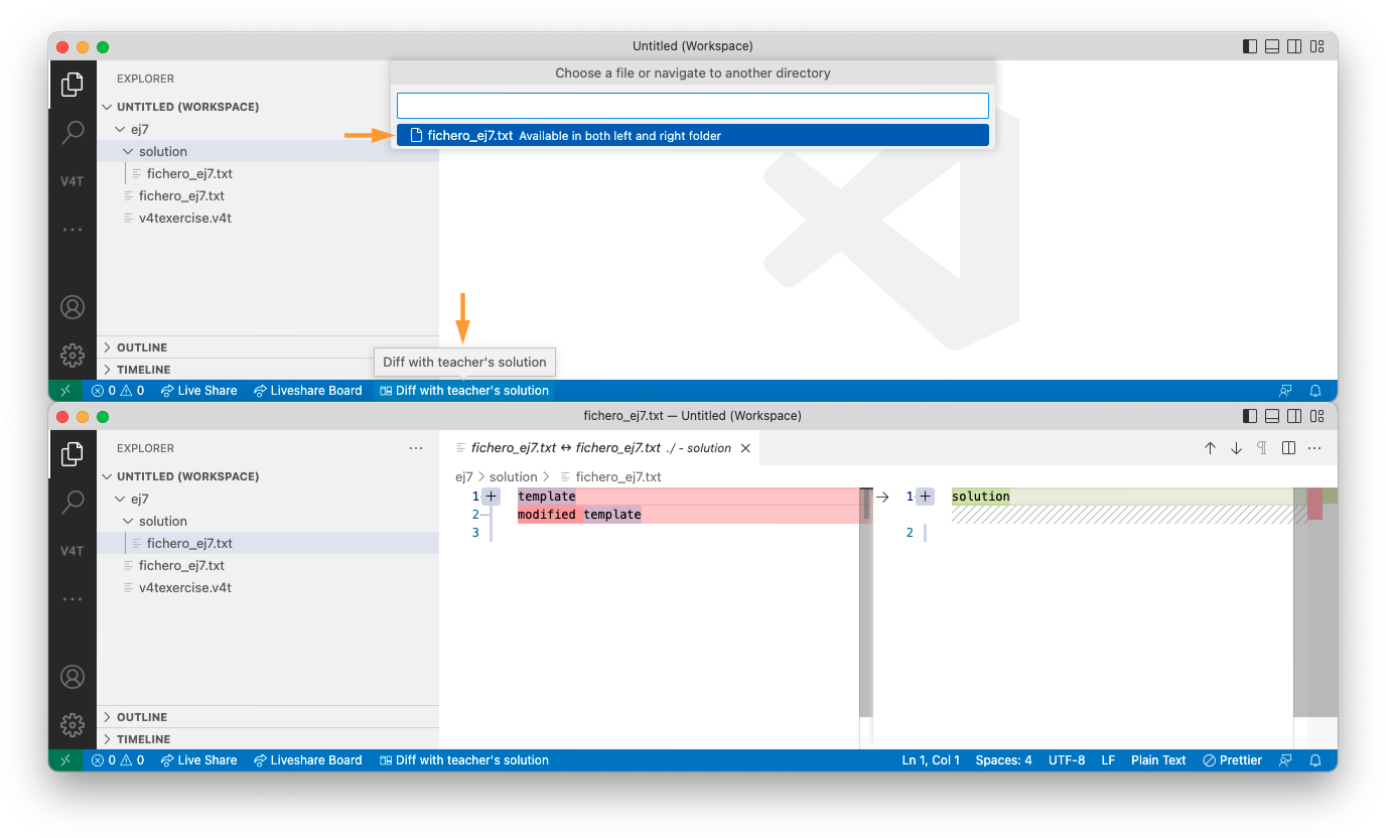
\includegraphics[width=\textwidth]{imagenes/utilizadas/4-3-implementacion/rf8-1.png}
    \caption{Captura de la extensión en la que se ejecuta la diferenciación entre la solución del docente y la propuesta del estudiante.}
    \label{fig:reqf8-1}
\end{figure}

\subsubsection{\texttt{RF-9}: página de ayuda personalizada}
\label{subsec:rf9}

Uno de los objetivos de la presente evolución de \textit{VSCode4Teaching} es el de favorecer una mejor interacción entre los usuarios y la aplicación, haciéndola más intuitiva y fácil de usar, tal como establece el punto cuarto de los objetivos establecidos en el \referenciaCapitulo{cap:objetivos}.

En las versiones previas de \textit{VSCode4Teaching} se implementó un formato de inscripción en los cursos con el siguiente flujo de operaciones asociado: el profesor disponía de un botón para generar un código de invitación para estudiantes, quienes debían introducirlo en un cuadro de diálogo con su sesión abierta en la extensión para matricularse en el curso. Este proceso puede resultar complejo si se carece de una explicación adecuada previa.

En línea con el objetivo establecido, se ha aprovechado la introducción de la nueva aplicación web ---véase la \referenciaSeccion{sec:diseñoArquitectura} a este respecto--- para crear una página de ayuda nueva. De este modo, de ahora en adelante, el profesor genera un enlace de invitación a una página web (y no únicamente un código) que los estudiantes reciben y abren en su navegador web, donde pueden encontrar una página de ayuda como la que se refleja en la \referenciaFigura{fig:reqf9-1}. Esta página muestra una primera invitación que varía según el código introducido, reflejando el nombre del profesor y del curso al que se ha invitado al alumno, pudiendo así garantizar \textit{a priori} que se ha recibido el enlace de invitación correcto. A continuación, se introduce una serie de imágenes animadas que permiten a los estudiantes tener un primer acercamiento con el funcionamiento de \textit{VSCode4Teaching} y familiarizarse con las funcionalidades que tienen disponibles. Además, en el punto en que se explica cómo inscribirse al curso haciendo uso del código, disponen de un campo especial con un botón que les permite copiar al portapapeles este código fácilmente.

\begin{figure}[ht]
    \centering
    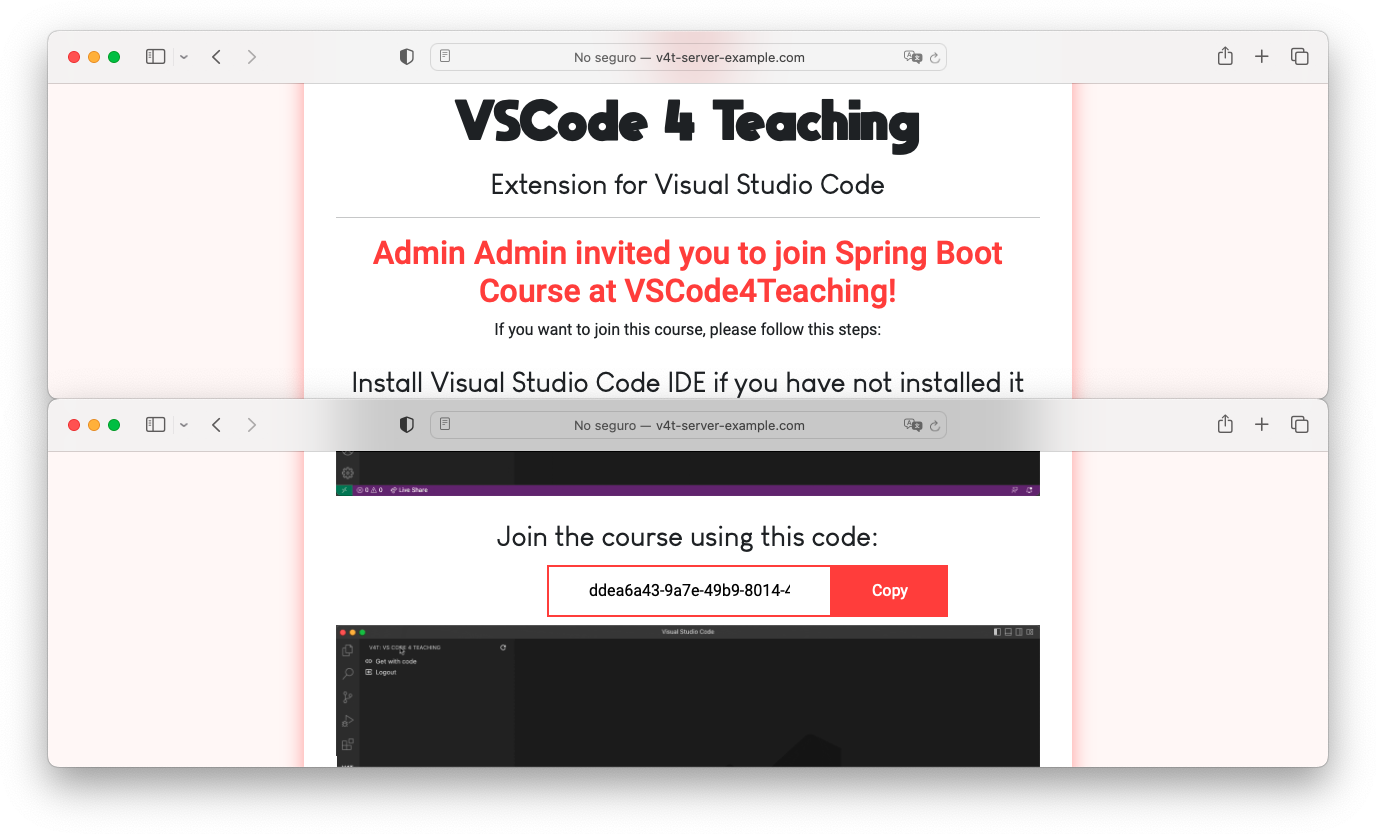
\includegraphics[width=\textwidth]{imagenes/utilizadas/4-3-implementacion/rf9-1.png}
    \caption{Captura de la página de ayuda personalizada según el código de invitación a curso suministrado.}
    \label{fig:reqf9-1}
\end{figure}

\subsubsection{\texttt{RF-10}: menú contextual en cursos}
\label{subsec:rf10}

En la extensión para Visual Studio Code, los usuarios pueden visualizar, con independencia de su rol, una lista de cursos y ejercicios. Los cursos tienen asociadas una serie de acciones ejecutables. Mientras que los estudiantes únicamente pueden refrescar el curso para actualizar sus ejercicios asociados, los docentes tienen disponibles las opciones para: compartir el enlace de invitación al curso, añadir nuevos ejercicios de forma simple o múltiple, inscribir o eliminar usuarios manualmente, refrescar la lista de ejercicios, modificar el nombre del curso o eliminarlo.

Todas estas acciones están asociadas a iconos. La ingente cantidad de iconos mostrados a los usuarios puede hacer que, hasta que no estén totalmente familiarizados con el uso de la aplicación, necesiten comprobar cuál es la finalidad de cada uno de ellos antes de accionarlos. Como consecuencia, en aras de una mejor interacción y con el fin de cumplir el segundo objetivo del TFG ---acerca de una mejor interacción usuario-aplicación, véase el \referenciaCapitulo{cap:objetivos}---, se ha implementado la posibilidad de visualizar un menú contextual que explica las acciones ejecutables mediante texto en lugar de iconos, haciéndolo más fácilmente comprensible, tal como se puede visualizar en la \referenciaFigura{fig:reqf10-1}. Para poder abrir este menú, los usuarios únicamente deben hacer \textit{click} secundario ---gesto habitualmente empleado para la apertura de este tipo de menús--- sobre un curso en la vista lateral de la extensión.

\begin{figure}[ht]
    \centering
    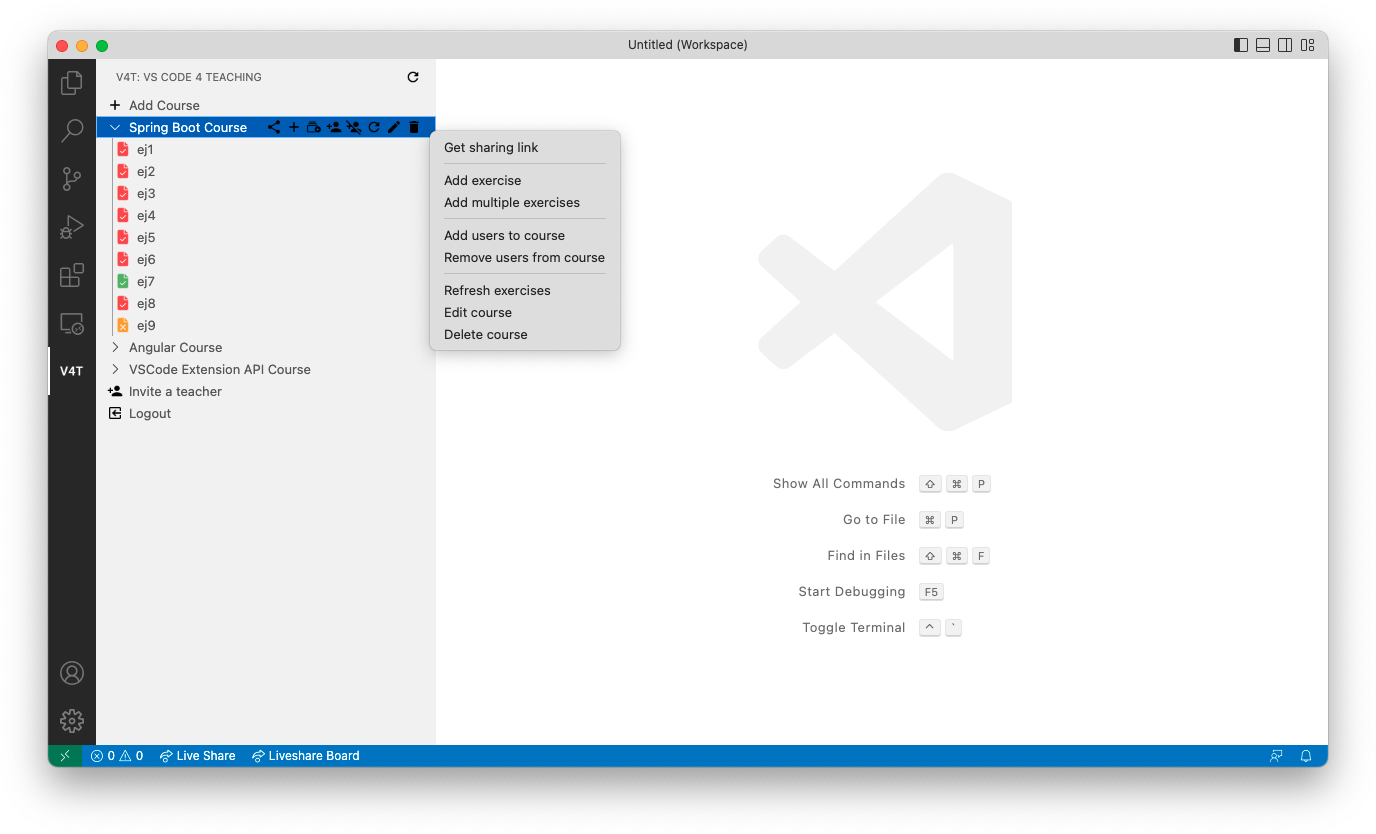
\includegraphics[width=\textwidth]{imagenes/utilizadas/4-3-implementacion/rf10-1.png}
    \caption{Menú mostrado a los docentes al hacer \textit{click} secundario sobre un curso.}
    \label{fig:reqf10-1}
\end{figure}

\subsubsection{\texttt{RF-11}: iconos de color para ejercicios}
\label{subsec:rf11}

Las aplicaciones que cuentan con GUI, como es el caso de \textit{VSCode4Teaching}, requieren que la interacción entre el usuario y los componentes que emplean sea lo más intuitiva y sencilla posible, buscando mostrar la información solicitada de forma clara y ágilmente interpretable, disponiendo los elementos necesarios para que el usuario actúe en consecuencia intercambiando nueva información con la aplicación, conduciendo a un uso fluido que satisfaga sus necesidades. Este hecho viene apoyado por el objetivo cuarto del Trabajo Fin de Grado ---véase el \referenciaCapitulo{cap:objetivos}---, que especifica que se deben incorporar mejoras visuales en la interfaz de usuario para facilitar el uso de la aplicación.

Gracias a la implementación del presente requisito, todos los usuarios de la aplicación ---con independencia de su rol--- visualizrán un nuevo icono junto a cada uno de los ejercicios disponibles.

Como la información que busca reflejar el icono es distinta para cada uno de los roles ---y, en consonancia, el propio icono---, se establecen dos requisitos derivados:
\begin{itemize}
    \item El requisito \texttt{RF-11.1} es el destinado a los estudiantes, estableciendo que el icono debe mostrar el estado en que se encuentra el ejercicio (pudiendo ser ``no comenzado'', ``en progreso'' o ``finalizado''). En la \referenciaFigura{fig:reqf11-1} se pueden apreciar los iconos mostrados a los estudiantes (en la parte izquierda): el ejercicio ``ej8'' tiene asociado el icono verde, asociado al último estado; ``ej9'', el icono amarillo ---reflejando estado ``en progreso''---; y ``ej7'', el icono rojo, que indica que el estudiante no ha comenzado el ejercicio.
    \item Análogamente, el requisito \texttt{RF-11.2} fija que los profesores visualicen un icono que aluda a la existencia de una solución adjunta al ejercicio y, en caso de haberla, que indique su disponibilidad. La \referenciaFigura{fig:reqf11-1} (en la parte derecha) ilustra los tres iconos disponibles para mostrar junto a cada ejercicio: el icono amarillo del ejercicio ``ej9'' indica que no tiene solución asociada; el rojo del ejercicio ``ej7'', que la solución adjunta no es pública; y el verde del ejercicio ``ej8'', que la solución ha sido publicada a los estudiantes.
\end{itemize}

Asimismo, la semántica de estos iconos también se refleja en el \textit{tooltip}\footnote{\textit{Tooltip}. Es un elemento textual que aparece en la interfaz de usuario cuando este mantiene el cursor encima de un ejercicio sin presionarlo durante varios segundos.}, en el que los estudiantes pueden visualizar entre paréntesis el estado del ejercicio en formato textual; y los docentes, una descripción sobre el estado de existencia y disponibilidad de la solución.

\begin{figure}[!ht]
    \centering
    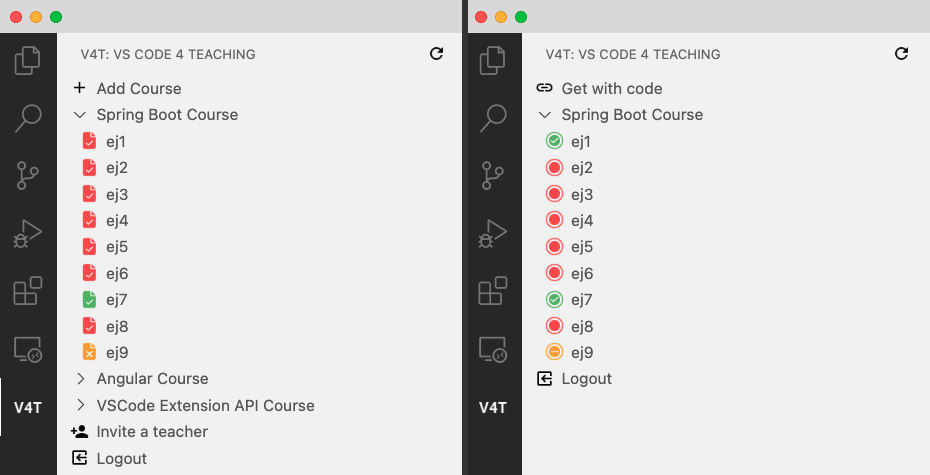
\includegraphics[width=\textwidth]{imagenes/utilizadas/4-3-implementacion/rf11-1.png}
    \caption{Iconos mostrados junto a cada ejercicio para los estudiantes (izquierda) y profesores (derecha).}
    \label{fig:reqf11-1}
\end{figure}

\subsubsection{\texttt{RF-12}: rediseño del \textit{dashboard}}
\label{subsec:rf12}

El cuarto objetivo del Trabajo Fin de Grado es lograr un mayor nivel de intuitividad en la extensión, potenciando la interacción entre usuario y aplicación mediante elementos de la GUI que permitan, entre otras finalidades, que los usuarios ---y, específicamente en este caso, los docentes--- reciban la información proporcionada por la extensión de una forma legible, visual y clara.

Las versiones previas de \textit{VSCode4Teaching} incorporaban un \textit{dashboard} que cumplía su función adecuadamente, ya que mostraba el progreso de los estudiantes en tiempo real, aportando para cada uno datos como nombre y apellidos, nombre de usuario, el tiempo transcurrido desde la última modificación y el estado del ejercicio; pero que contaba con una estética poco desarrollada y que no mostraba métricas como, por ejemplo, la cantidad de alumnos que no habían comenzado aún el ejercicio o cuántos lo habían finalizado ya. Esta versión del \textit{dashboard} puede ser visualizada en la \referenciaFigura{fig:reqf12-1}.

\begin{figure}[ht]
    \centering
    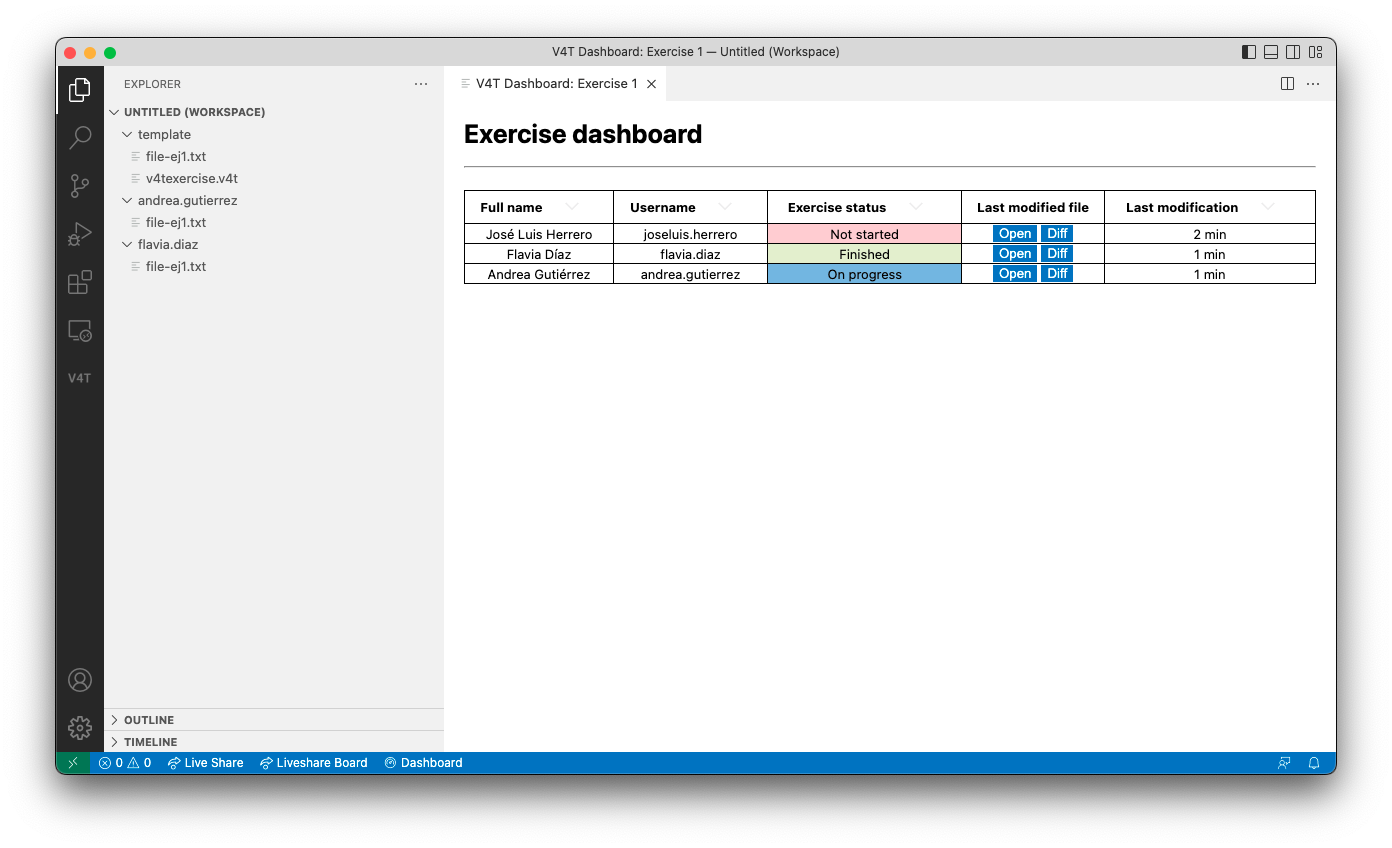
\includegraphics[width=0.925\textwidth]{imagenes/utilizadas/4-3-implementacion/rf12-1.png}
    \caption{Captura del \textit{dashboard} de \textit{VSCode4Teaching} previa a su modificación visual.}
    \label{fig:reqf12-1}
\end{figure}

\begin{figure}[ht]
    \centering
    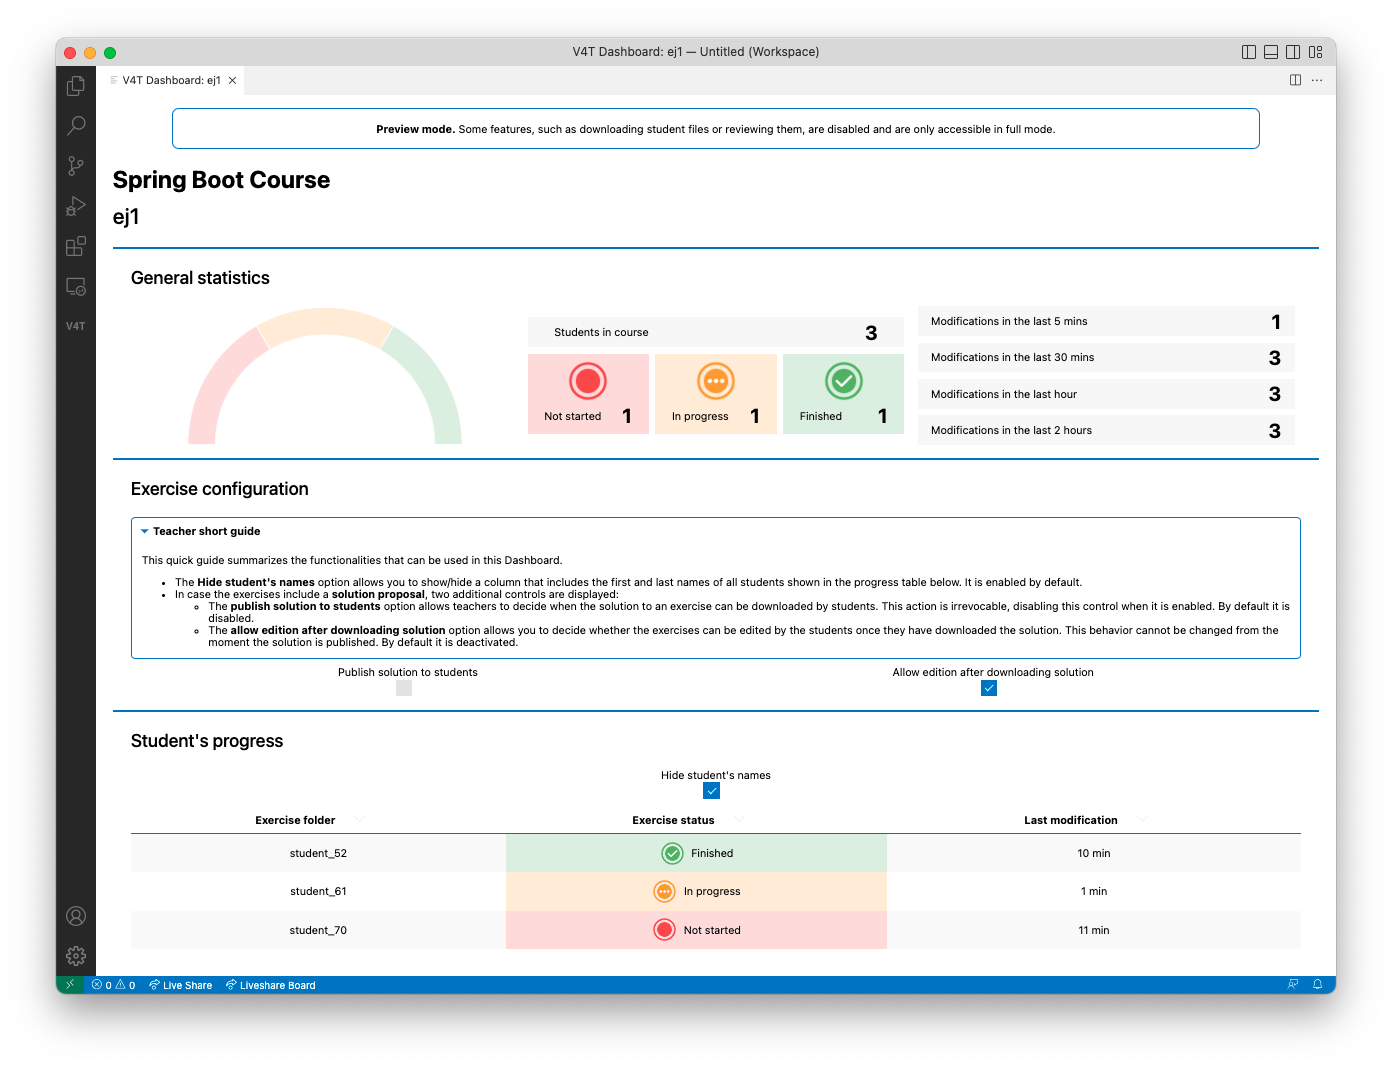
\includegraphics[width=0.925\textwidth]{imagenes/utilizadas/4-3-implementacion/rf12-2.png}
    \caption{Instantánea del \textit{dashboard} de \textit{VSCode4Teaching} tras su rediseño.}
    \label{fig:reqf12-2}
\end{figure}

Unificando el objetivo cuarto del proyecto \textit{VSCode4Teaching} ---véase \referenciaCapitulo{cap:objetivos}--- con la necesidad de generar una estética mejor y más funcional para el \textit{dashboard}, se ha ejecutado una labor de rediseño basada en tres ejes principales: la introducción de un gráfico semicircular que muestra la evolución del conjunto de estudiantes en la realización del ejercicio y la proporción de estudiantes que hay en cada uno de sus posibles estados, la introducción de nuevos parámetros estadísticos basados en el recuento de estudiantes presentes en cada uno de los estados del ejercicio y en la consideración del tiempo transcurrido en bloques de 5, 30, 60 y 120 minutos y la introducción de una guía de ayuda a docentes para explicar rápida y concisamente la funcionalidad de cada uno de los elementos de control y configuración presentes en el \textit{dashboard}.

Se introduce una instantánea del nuevo \textit{dashboard} en la \referenciaFigura{fig:reqf12-1} que, por comparación con la \referenciaFigura{fig:reqf12-2}, permite evidenciar la evolución introducida y la labor de rediseño ejecutada en una nueva visualización que cuenta con tres secciones claramente diferenciadas: una de estadísticas generales, en la que se introducen los nuevos elementos gráficos citados con anterioridad, otra de configuración en la que los docentes pueden acceder a la guía rápida y a la configuración sobre la solución ---en caso de haberla--- y una sección de progreso individual de los estudiantes, que muestra una tabla de estética mejorada con la información y funcionalidad que venía estando disponible en versiones anteriores.


\subsection{Requisitos no funcionales}
\label{subsec:reqsNoFuncionales}
\subsubsection{\texttt{RN-1}: ciberseguridad y mantenimiento preventivo}
\label{subsec:rn1}

La ciberseguridad es la ``práctica de proteger sistemas, redes y programas de ataques digitales [...] que apuntan a acceder, modificar o destruir la información confidencial, extorsionar a los usuarios o interrumpir la continuidad del negocio'' \cite{rn1_queEsCiber}.

De esta definición se extrapola el papel fundamental que la seguridad informática ocupa en el desarrollo y mantenimiento de todos los programas, generando un trabajo constante y necesario de detección y solución de problemas en materia de confidencialidad, integridad y disponibilidad ---los pilares básicos de la seguridad informática--- de las herramientas informáticas y los datos que involucran en su uso.

Durante el desarrollo de este Trabajo Fin de Grado, han sido detectadas numerosas vulnerabilidades en las dependencias y \textit{frameworks} empleados para la implementación de \textit{VSCode4Teaching}, condición suficiente para la introducción de cuatro \textit{sprints} o pequeños periodos de tiempo dedicados específicamente a la actualización de estas librerías a sus últimas versiones disponibles.

El servidor ha sido el más afectado por las vulnerabilidades surgidas en los últimos meses. Alrededor de este componente, que se basa en el uso del \textit{framework} Spring ---véase \referenciaSeccion{subsec:tecServidor} para más información---, han aparecido importantes vulnerabilidades. Algunas de las más destacadas han sido catalogadas en la lista \textit{Common Vulnerabilities and Exposures} (CVE\footnote{CVE. Siglas de ``vulnerabilidades y revelaciones comunes'' (del inglés \textit{Common Vulnerabilities and Exposures}). Es una de las listas de recopilación de vulnerabilidades y riesgos de seguridad más extendidas actualmente.}) \cite{rn1_cve} como: CVE-2021-44228, CVE-2021-45046, CVE-2021-45105 (noviembre-diciembre 2021, conocidas como ``Log4j'') y CVE-2022-22965 (enero 2022, conocida como ``Spring4Shell''). Como consecuencia, se ha introducido una actualización de la versión de Spring Boot a la más reciente disponible en la fecha de cierre del trabajo (2.7.5), así como de las dependencias empleadas para el funcionamiento del servidor.

Asimismo, sobre la extensión para Visual Studio Code se han ejecutado actualizaciones de dependencias y \textit{frameworks} para introducir correcciones a vulnerabilidades como las identificadas como CVE-2021-3918 (noviembre 2021), CVE-2021-44906 (diciembre 2021) o CVE-2022-0155 (enero 2022), así como actualizaciones de las diversas librerías empleadas a las últimas versiones divulgadas.

La aplicación web SPA también ha recibido diversas actualizaciones, aplicadas tanto a su \textit{framework} de base, Angular (actualizado a versión 14.2.11) como a alguna de sus dependencias por motivo de mejora en materia de seguridad y de rendimiento.

\subsubsection{\texttt{RN-2}: sistemas de registro de eventos}
\label{subsec:rn2}

La mantenibilidad es uno de los atributos de calidad esenciales en todos los proyectos \textit{software}, especialmente en aquellos con naturaleza de código libre como \textit{VSCode4Teaching}. Es por ello que resulta crucial introducir requisitos que permitan dar una evolución y mantenimiento adecuados a las aplicaciones para poder ejecutar desarrollos posteriores de forma más sencilla y rápida. Una de estas herramientas son los sistemas de registro de eventos o \textit{logs} y que permiten a los desarrolladores depurar y comprender el funcionamiento de las aplicaciones de forma más adecuada en tiempo real mientras funcionan, dejando constancia escrita de aquellas acciones que se deseen registrar a medida que suceden durante el uso de la aplicación.

\textit{VSCode4Teaching} introduce sistemas de registro de eventos en sus tres componentes, potenciando el uso de los anteriormente existentes e incorporando nuevas librerías que permiten organizarlos de forma más adecuada. El servidor introduce la biblioteca \textit{Log4J} \cite{rn2_tecLogServidor}, que está integrada dentro del \textit{framework} Spring en el que se basa ---tal como queda reflejado en la \referenciaSeccion{subsec:tecServidor}---, potenciando su utilización mediante la revisión de los eventos inventariados anteriormente existentes y la introducción de registros de actividades como la recepción y gestión de peticiones y el envío de sus respectivas respuestas.

Por otro lado, la extensión introduce la librería \textit{Winston} \cite{rn2_tecLogExtension} con el mismo propósito, permitiendo generar una traza de las peticiones que, cotejándolo con el registro anteriormente comentado, permite analizar su interacción con el servidor, recogiendo las peticiones enviadas y recibidas, las demoras temporales que se producen o el estado del cuerpo de las peticiones en su envío y en su recepción.

Asimismo, aunque su utilización es menor, también se introduce en la aplicación web SPA la librería \textit{ngx-logger} \cite{rn2_tecLogAppWeb} y se reflejan registros de las peticiones que envía al servidor durante los procesos de usuario ejecutados en este componente.

\subsubsection{\texttt{RN-3}: generación de imagen Docker}
\label{subsec:rn3}

Tal como queda recogido en la \referenciaSeccion{sec:distribDespliegue}, el servidor de \textit{VSCode4Teaching} está preparado para ser compilado en formato de imagen Docker, permitiendo de este modo la ejecución de instancias del servidor en forma de contenedores ligeros sobre cualquier sistema operativo, añadiendo la portabilidad a la lista de atributos de calidad del proyecto.

Docker se sirve de pequeños ficheros de configuración conocidos como \textit{Dockerfile} \cite{rn3_dockerfile}, que se introducen en la raíz de los proyectos y contienen las instrucciones necesarias para, a partir del código fuente, generar la imagen divulgable e instanciable de la aplicación. En el \referenciaCodigo{cod:dockerfileAnterior} se observa la versión original del fichero \textit{Dockerfile}, que requería de la existencia previa de un artefacto JAR del servidor.

Debido a la introducción de la nueva aplicación web SPA ---véase la \referenciaSeccion{sec:diseñoArquitectura}---, que queda compilada y embebida en el servidor antes de generar su imagen, y a la necesidad de poder compilar la imagen en cualquier computador sin necesidad de que tenga instalado ninguna herramienta adicional al propio Docker, se ha rediseñado y ampliado esta configuración para que la compilación se logre a partir de la ejecución de tres pasos en cascada que quedan definidos en un fichero \textit{multi-stage}\footnote{\textit{Multi-stage}. En la generación de imágenes Docker, se dice que un fichero de configuración es \textit{multi-stage} cuando requiere de la ejecución de varias fases en contenedores distintos para crear una imagen.} \cite{rn3_multistage}, tal como queda reflejado en el \referenciaCodigo{cod:dockerfileNuevo}: compilación de la aplicación Angular, compilación del servidor con la aplicación Angular compilada embebida y generación de la imagen final apta para la ejecución del JAR obtenido.

\begin{lstlisting}[language=Dockerfile,caption={\textit{Dockerfile} original del proyecto.},label=cod:dockerfileAnterior]
FROM adoptopenjdk/openjdk11:latest
RUN apt-get update && apt-get install -y netcat && rm -rf /var/lib/apt/lists/*
COPY ./target/vscode4teaching-server-*.jar ./app/vscode4teaching-server-*.jar
COPY ./docker/waitDB.sh ./app/waitDB.sh
EXPOSE 8080
RUN ["chmod", "+x", "./app/waitDB.sh"]
CMD ["./app/waitDB.sh"]
\end{lstlisting}

\begin{lstlisting}[language=Dockerfile,caption={\textit{Dockerfile} actualizado para introducir la compilación independiente del sistema operativo y de la aplicación web.},label=cod:dockerfileNuevo]
# Step 1: Compilation of Angular frontend
# It will be embedded as a static resource into Spring Boot backend
FROM node:16.13.2 AS angular
COPY vscode4teaching-webapp /usr/src/app
WORKDIR /usr/src/app
RUN ["npm", "install"]
RUN ["npm", "run", "build"]
# Step 2: Compilation of Maven project (generation of JAR)
FROM maven:3.8.4-jdk-11 AS builder
COPY vscode4teaching-server /data
COPY --from=angular /usr/src/app/dist /data/src/main/resources/static
WORKDIR /data
RUN ["mvn", "clean", "package"]
# Step 3: Generation of Docker image using the JAR previously built
FROM adoptopenjdk/openjdk11:latest
RUN apt-get update && apt-get install -y netcat && rm -rf /var/lib/apt/lists/*
COPY --from=builder /data/target/vscode4teaching-server-*.jar ./app/vscode4teaching-server-*.jar
COPY vscode4teaching-server/docker/waitDB.sh ./app/waitDB.sh
EXPOSE 8080
RUN ["chmod", "+x", "./app/waitDB.sh"]
CMD ["./app/waitDB.sh"]
\end{lstlisting}

Se introducen, además, ficheros \texttt{.dockerignore} \cite{rn3_dockerfile}, que permiten especificar adecuadamente qué ficheros pueden ser ignorados para compilar los componentes correctamente, permitiendo una rebaja en la cantidad de almacenamiento y recursos del computador empleados durante el proceso.
\subsubsection{\texttt{RN-4}: documentación de API REST}
\label{subsec:rn4}

Con la misma vocación de mantenibilidad que el requisito \texttt{RN-2} ---detallado en la \referenciaSeccion{subsec:rn2}---, el presente requerimiento busca potenciar la documentación del proyecto \textit{VSCode4Teaching}, entendiendo que este es uno de los pilares esenciales que permite a todos los desarrolladores ---con independencia de si pertenecen al proyecto o no--- comprender de forma sencilla y ágil el funcionamiento de la aplicación y la organización y aspecto del código fuente que lo conforma.

La API REST es el ``eje vertebrador'' que da unidad a \textit{VSCode4Teaching}, tal como se evidencia en la \referenciaSeccion{sec:diseñoArquitectura}, que introduce una disquisición exhaustiva sobre la organización de la aplicación que manifiesta, entre otros rasgos significativos, que esta API es la que permite la comunicación e interacción entre el servidor y los clientes de la aplicación, siendo el canal de comunicación de información bidireccional establecido entre los citados componentes.

Con el fin de potenciar la documentación existente en el proyecto sobre esta API, se ha introducido \textit{Swagger}, que es una tecnología que permite ``simplificar el desarrollo de APIs para usuarios, equipos y corporaciones con una plataforma de código abierto'' \cite{rn4_swagger}, que toma las declaraciones de \textit{endpoints} disponibles en el código fuente del servidor para generar su documentación automáticamente en el formato estipulado en el estándar \textit{OpenAPI}, que fue creado por un ``consorcio de [...] expertos que reconoce el inmenso valor de estandarizar cómo se describen las APIs''\cite{rn4_openapi} y que es uno de los más extendidos en la actualidad. Adicionalmente, permite la visualización gráfica de la documentación generada en un entorno intuitivo a través de cualquier navegador web haciendo uso de la herramienta \textit{Swagger UI} \cite{rn4_swaggerui}, tal como puede visualizarse en la \referenciaFigura{fig:reqn4-1}. Gracias a la incorporación de esta herramienta, se introduce en el código fuente del servidor la documentación en formato JSON según el estándar \textit{OpenAPI} de la API REST implementada, viéndose actualizado concordantemente con la modificación o ampliación de la implementación de los \textit{endpoints} que integran la API de este servidor.

\begin{figure}[ht]
    \centering
    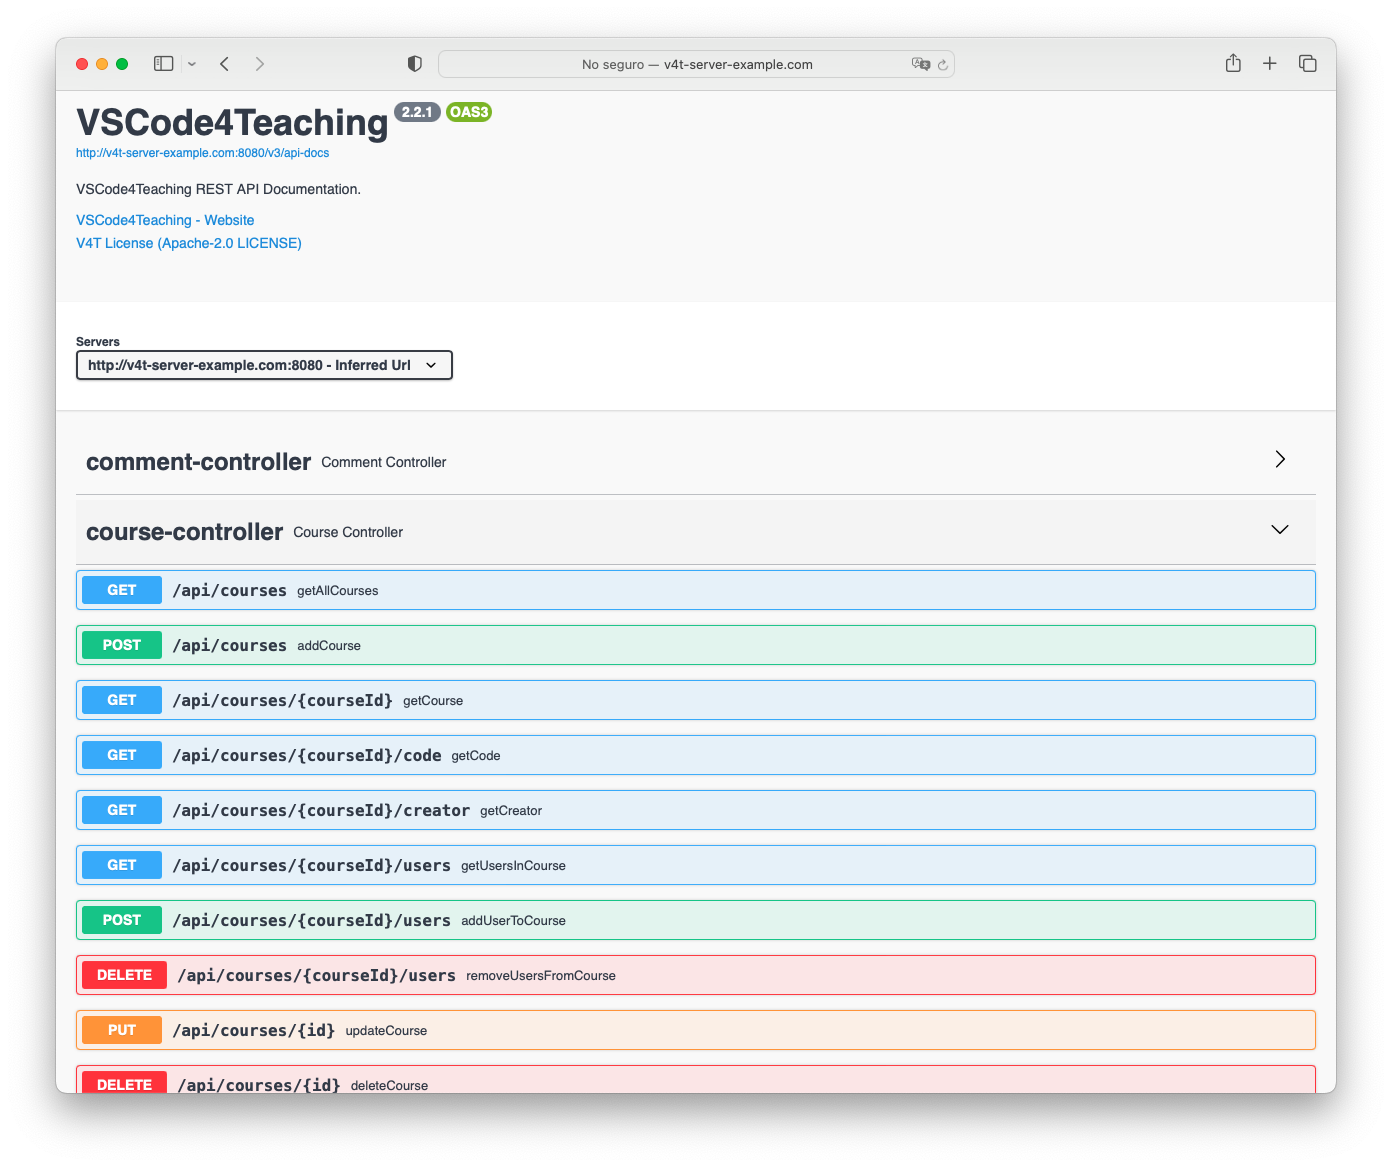
\includegraphics[width=\textwidth]{imagenes/utilizadas/4-3-implementacion/rn4-1.png}
    \caption{Vista de \textit{Swagger UI} mostrando los \textit{endpoints} disponibles en la API de VSCode4Teaching en un navegador web.}
    \label{fig:reqn4-1}
\end{figure}


\subsection{Requisitos de corrección de errores}
\label{subsec:reqsErrores}
Una vez inician su explotación ---es decir, su utilización habitual por parte de los usuarios---, las aplicaciones informáticas comienzan a registrar errores existentes en el flujo de uso, procedentes tanto de errores en la implementación de alguno de los componentes de la aplicación como de fallos en la comunicación entre ellos.

Tal como se desarrolla en la \referenciaSeccion{sec:metodologia}, la detección y corrección de errores se ha ejecutado paralelamente al desarrollo e incorporación de los demás requisitos descritos con anterioridad, ejecutando iteraciones de diagnóstico y solución de errores en tres fases: triaje del error, realizando una ``anamnesis'' para determinar las condiciones en las que se producía el error ---cuándo se producía, si se derivaba de alguna acción específica de los usuarios de un cierto rol, si sucedía periódicamente o cuáles eran las consecuencias derivadas de su ocurrencia, entre otras, con el fin de recolectar toda la información posible acerca del error---; primera implementación de una corrección, haciendo las modificaciones oportunas en el código fuente de los componentes involucrados para tratar de corregir el error; y verificación de la corrección, reproduciendo las condiciones en las que se produjo el error originalmente y evaluando si se vuelve a producir, si se produce algún otro error derivado de la corrección o si se ha subsanado en su totalidad.

El descubrimiento de nuevos errores para su posterior corrección se ha ejecutado a través de las pruebas realizadas para la verificación del \textit{software}, que se ven descritas en la \referenciaSeccion{sec:verificacion}. Las pruebas implementadas sobre el código ---esto es, las pruebas unitarias y de integración--- han permitido detectar errores lógicos mediante la comparación de resultados esperados frente a resultados obtenidos, dando lugar a algunos requisitos como el \texttt{RE-1}.
Por otro lado, las pruebas de uso en simulaciones de entornos reales han permitido encontrar fallos en la aplicación a través de la imitación de potenciales flujos de uso habituales en entornos en explotación; esto es, recreando acciones y comportamientos de usuarios, encontrando fallos que las pruebas de código implementadas para este proyecto no permiten localizar, como pueden ser los requisitos \texttt{RE-4} o \texttt{RE-6}.

Tal como se introducía en la \referenciaSeccion{subsec:listaReqsErrores}, cabe reseñar seis requisitos de entre todas las correcciones de errores ejecutados en el proyecto \textit{VSCode4Teaching}:
\begin{itemize}
    \item \texttt{\textbf{RE-1}}. Los profesores disponen de una tabla en el \textit{dashboard} para visualizar el progreso individualizado de los estudiantes en la realización de los ejercicios propuestos. Esta tabla tiene controles que permiten la ordenación de sus filas alfabéticamente según los valores de cada una de las columnas. Cuando se pretendía ordenar la tabla del \textit{dashboard} según alguna columna, el resultado de la ordenación mostrado era incorrecto, pudiendo ser ordenados por los valores de columnas diferentes o de forma aparentemente arbitraria.
    \item \texttt{\textbf{RE-2}}. Los profesores tienen a su disposición una funcionalidad para añadir varios ejercicios simultáneamente en un determinado curso. Cuando la empleaban, aparecía un directorio intermedio no existente en origen con el mismo nombre en el que se introducían todos los contenidos del ejercicio, que se mostraban en un nivel superior cuando se agregaban de uno en uno, de modo que el comportamiento de la funcionalidad daba resultados diferentes según si se ejecutaba para ejercicios individuales o para grupos de ejercicios.
    \item \texttt{\textbf{RE-3}}. Los estudiantes pueden tener los ejercicios de los cursos en los que participan en distintos estados: ``no comenzado'', cuando aún no han abierto los ejercicios en su editor de código; ``en progreso'', cuando han accedido al ejercicio en su editor; y ``finalizado'', cuando, una vez han realizado modificaciones, deciden marcarlo como finalizado, bloqueando sucesivas ediciones de su propuesta de resolución del ejercicio. Las pruebas de simulación de entornos reales permitieron detectar algunos errores que impedían que la extensión siguiese adecuadamente el progreso de los estudiantes al no modificar el estado a ``en progreso'' al comenzar el ejercicio, de modo que las modificaciones realizadas no quedaban almacenadas en el servidor. Además, una vez que los estudiantes marcaban como finalizados los ejercicios, en caso de que los descargasen de nuevo, veían revertido su estado a ``en progreso'', permitiéndoles volver a editar sus propuestas de resolución una vez marcadas como finalizadas.
    \item \texttt{\textbf{RE-4}}. En la tabla que se muestra a los profesores en el \textit{dashboard}, uno de los datos que quedan reflejados es la fecha de última modificación realizada por cada uno de los estudiantes. Este dato refleja cuánto tiempo ha transcurrido desde la última modificación registrada en base de datos, actualizándose periódicamente para reflejar valores correctos mientras se mantenga abierta esta visualización. En una prueba de simulación de entorno real se descubrió que una modificación en la interfaz de usuario de esta visualización provocó que la rutina periódica tuviese una configuración inadecuada, readaptándose para su correcta visualización en posteriores ediciones.
    \item \texttt{\textbf{RE-5}}. Cuando se producen cierres de sesión en la extensión de \textit{VSCode4Teaching}, es preciso ocultar y deshabilitar todas las funciones propias de los usuarios autenticados, ya que su utilización posterior al fin de la autenticación puede entrañar un riesgo de seguridad, pues los elementos de la interfaz de usuario que permiten la ejecución de funcionalidades como, por ejemplo, la visualización del \textit{dashboard}, de acceso restringido a profesores, quedaban visibles y funcionales en la GUI. Para eliminar este error, se introducen nuevos controles que dotan a la extensión de capacidades para eliminar todos los elementos de la interfaz que solo pueden ser ejecutados por usuarios identificados en la extensión.
    \item \texttt{\textbf{RE-6}}. Las pruebas realizadas en simulación de entornos reales permiten también detectar problemas de rendimiento y carga de la aplicación, tal como se desarrolla en la \referenciaSeccion{subsec:pruebasManuales}. Uno de los errores producidos como consecuencia de un problema de estas características se manifiesta ante la ejecución de la funcionalidad de la que los profesores disponen para cargar ejercicios de forma masiva en sus cursos. Anteriormente, se enviaban todas las peticiones para la subida de plantillas y propuestas de solución (en caso de haberlas) de forma simultánea desde la petición, ocasionando que el servidor recibiese una alta cantidad de peticiones a la vez, hecho que provocaba el incorrecto procesamiento de los ejercicios. Se ha introducido una modificación para hacer que la extensión envíe las peticiones de forma secuencial, lanzando una nueva petición cada vez que se recibe confirmación del servidor a la inmediatamente anterior, mitigando el problema de carga del servidor.
\end{itemize}

